\section{Gaussian reduction and a hard-boundary tail}
\label{sec:preparation}
This section retains the model and the order of limits of
Section~\ref{sec:logtime}. We now distinguish two early-time laws for
the \emph{limiting} correlator. The exponent two for an unprojected
semiclassical OTOC is already present in KL; here we check the fixed
Gaussian preparation explicitly. The hard moving threshold gives a
different result for the specific density $\pi_0(r)=\beta e^{-\beta r}$,
$\beta>0$. No finite-$M$ growing-window error estimate is supplied.

\subsection{A factorization of the surviving branch}
Change coordinates to
\begin{equation}
 \chi=x-y+z,\quad u=x-\chi/2,\quad v=z-\chi/2,
 \qquad y=u+v,
 \label{eq:prep-coordinates}
\end{equation}
with absolute Jacobian one. Define
\begin{align}
 f_\chi(w)&=e^{-\pi w-\sigma^2w^2}
   \prod_{\epsilon=\pm1}\prod_{\eta=\pm1}
   \Gamma\left(\frac14+\frac{i\chi}{4}
                    +\frac{i\eta}{2}(w+\epsilon\nu)\right),\notag\\
 J(\chi)&=\int_{\mathbb R}f_\chi(w)\dd w,\qquad
 K=\frac{J(0)}{16\pi^3}=\int_{\mathbb R}k(w)\dd w.
 \label{eq:prep-f-J}
\end{align}
For real $\chi$, direct cancellation of the eight external Gamma
factors against $V_-$ gives
\begin{equation}
 \frac{H_\nu V_-}{\pi^3}e^{-\sigma^2Q/2}
 =\frac{2^{2i\chi}\cosh(\pi\chi/2)}{512\pi^7}
       e^{-\sigma^2\chi^2/2}f_\chi(u)f_\chi(v).
 \label{eq:prep-factorization}
\end{equation}
For example the $x$-dependent numerator of the $c$ ratios in $V_-$
is $c(1/2-i(x+\nu))c(1/2-i(x-\nu))$; its denominator replaces
$x$ by $x-\chi$. Inserting the defining Gamma ratios cancels precisely
the oppositely oriented two external edges. The remaining $x$ and $z$
factors are equal after \eqref{eq:prep-coordinates}. Also
$Q=2u^2+2v^2+\chi^2$. This verifies the phase $2^{2i\chi}$ and all
normalizations without dropping external phases.

For the fixed threshold this gives the one-dimensional Fourier integral
\begin{align}
 \mathcal X_F(T)&=\frac{K^2}{2}
                  +\operatorname{PV}\int_{\mathbb R}e^{iT\chi}
                         A_F(\chi)\dd\chi,\notag\\
 A_F(\chi)&=\frac{2^{2i\chi}}{512\pi^7}
  \Gamma(-i\chi)\cosh(\pi\chi/2)e^{-\sigma^2\chi^2/2}J(\chi)^2.
 \label{eq:prep-fixed-Fourier}
\end{align}
Only the scalar integral defining $J$ remains inside the Fourier
integral. Near zero $A_F=iK^2/(2\pi\chi)+O(1)$. Thus a useful
ordinary-integral implementation is
\begin{equation}
 \mathcal X_F(T)=\frac{K^2}{2}\,[1-\operatorname{erf}(T/2)]
  +\int_{\mathbb R}e^{iT\chi}
    \left[A_F(\chi)-\frac{iK^2e^{-\chi^2}}{2\pi\chi}\right]\dd\chi.
 \label{eq:prep-subtracted}
\end{equation}
The bracket has a removable value at zero. Real-axis conjugation gives
$A_F(-\chi)=\overline{A_F(\chi)}$, hence $\mathcal X_F(T)$ is real.

\subsection{Fixed threshold: the first surviving pole}
\begin{theorem}[Gaussian fixed-threshold early asymptotic]
For fixed $\nu,\sigma>0$ and any $2<h<4$,
\begin{align}
 \mathcal X_F(T)&=K^2-C_{\nu,\sigma}e^{2T}+O_h(e^{hT}),\notag\\
 \mathcal D_F(T)&=2C_{\nu,\sigma}e^{2T}+O_h(e^{hT}),
 \qquad T\to-\infty,\notag\\
 C_{\nu,\sigma}&=\frac{e^{2\sigma^2}}{32\pi^6}J(-2i)^2>0.
 \label{eq:prep-fixed-early}
\end{align}
The constants are not asserted uniform as $\sigma\to0$ or $\infty$.
\label{thm:prep-fixed}
\end{theorem}
\begin{proof}
In the closed lower strip $-h\le\operatorname{Im}\chi\le0$, the real
part of every Gamma argument in \eqref{eq:prep-f-J} is between $1/4$
and $1/4+h/4$. Euler's integral bounds their moduli and all fixed
parameter derivatives by constants uniform in the imaginary arguments.
The $w$ Gaussian therefore gives holomorphy of $J$ and a uniform bound
on each such strip. The Gamma asymptotic on vertical lines then bounds
\(\Gamma(-i\chi)\cosh(\pi\chi/2)\) by a polynomial in
$|\operatorname{Re}\chi|$ away from its poles. The remaining Gaussian
ensures horizontal integrability and vanishing vertical sides.

The odd poles cancel, as is manifest in the identity
\begin{equation}
 \Gamma(-i\chi)\cosh(\pi\chi/2)
  =2^{-i\chi-1}\sqrt\pi\,
       \frac{\Gamma(-i\chi/2)}{\Gamma((1+i\chi)/2)}.
 \label{eq:prep-even-poles}
\end{equation}
Move the principal-value contour down to $\mathbb R-ih$. Clockwise
orientation gives minus one half of $2\pi i$ times the zero-pole
residue, and minus $2\pi i$ times each pole strictly below it. The zero
pole adds $K^2/2$. The only other pole crossed is $\chi=-2i$, with
\[
 \operatorname*{Res}_{\chi=-2i}A_F
   =-\frac{i e^{2\sigma^2}J(-2i)^2}{64\pi^7}.
\]
This yields the negative coefficient in \eqref{eq:prep-fixed-early}.
On the displaced line $|e^{iT\chi}|=e^{hT}$ and its remaining integral
is absolutely bounded. Finally
\[
 J(-2i)=\int_{\mathbb R}e^{-\pi w-\sigma^2w^2}
       \prod_{\epsilon=\pm1}
       \left|\Gamma\left(\frac34+\frac i2(w+\epsilon\nu)\right)\right|^2
       \dd w>0.
\]
Since $N^F_\infty=K^2$, the commutator formula follows.
\end{proof}
This is an exponent for the ordered limit $M\to\infty$ followed by
$T\to-\infty$ of the specified vacuum commutator norm. It is not,
without a uniform finite-$M$ remainder, a fitted Lyapunov exponent over
an arbitrary experimental time window.

\subsection{Moving threshold: an explicit corner contribution}
For $\pi_0(r)=\beta e^{-\beta r}$, retain the hard projection at each
insertion. Define
\begin{align}
 J_Q(\chi)&=\int_0^\infty\beta e^{-\beta r}\dd r
       \iint_{D_{r,\chi}}f_\chi(u)f_\chi(v)\dd u\dd v,\notag\\
 D_{r,\chi}&=\{u,v\ge-r-\chi/2,\ u+v\ge-r\}.
 \label{eq:prep-moving-domain}
\end{align}
For real $\chi$ this is an ordinary convergent integral. Replacing
$J^2$ by $J_Q$ in $A_F$ defines $A_Q$, and
\begin{equation}
 \mathcal X_Q(T)=\frac{X^Q_\infty}{2}
            +\operatorname{PV}\int e^{iT\chi}A_Q(\chi)\dd\chi,
 \qquad X^Q_\infty=\frac{J_Q(0)}{256\pi^6}.
 \label{eq:prep-moving-Fourier}
\end{equation}
The regularity proved next justifies this ordinary PV for the exponential
density; it does not assert it for every $L^1$ density of Section~12.

Put $a=-r-\chi/2$, $L=r+\chi$ and
\begin{align}
 B(r,\chi)&=\int_{s,t\ge0,\ s+t<1}
       f_\chi(a+Ls)f_\chi(a+Lt)\dd s\dd t,\notag\\
 I(r,\chi)&=\left[\int_a^\infty f_\chi(w)\dd w\right]^2
                  -L_+^2 B(r,\chi).
 \label{eq:prep-triangle}
\end{align}
Indeed the square of half-lines has a triangular forbidden region only
when $L>0$. If the factor $L_+^2$ is replaced by $L^2$, the resulting
$r$ integral is a smooth function $J_{\rm sm}(\chi)$ on the real line.
The exact difference is
\begin{equation}
 J_Q(\chi)-J_{\rm sm}(\chi)
 =\one_{\chi<0}\int_0^{-\chi}\beta e^{-\beta r}
                     (r+\chi)^2 B(r,\chi)\dd r
 =\frac{\beta f_0(0)^2}{6}(-\chi)_+^3
       +O\bigl(({-\chi})_+^4\bigr).
 \label{eq:prep-corner}
\end{equation}
The Taylor remainder here also has the one-sided derivative bounds
obtained by differentiating the rescaled simplex integral. In particular
it is not merely a pointwise big-$O$ assertion.

\begin{theorem}[Hard-boundary inverse-cubic tail]
For the stated exponential density, fixed $\beta,\nu,\sigma>0$, define
\begin{equation}
 B_{\beta,\nu}=\frac{\beta f_0(0)^2}{1536\pi^7}
   =\frac{\beta|\Gamma(1/4+i\nu/2)|^8}{1536\pi^7}>0.
 \label{eq:prep-cubic-coefficient}
\end{equation}
In the order of limits specified above,
\begin{align}
 \mathcal X_Q(T)&=X^Q_\infty+\frac{B_{\beta,\nu}}{T^3}
                           +O(|T|^{-4}),&&T\to-\infty,\notag\\
 \mathcal X_Q(T)&=\frac{B_{\beta,\nu}}{T^3}
                           +O(T^{-4}),&&T\to+\infty,\notag\\
 \mathcal D_Q(T)-\mathcal D_{\rm edge}
     &=\frac{2B_{\beta,\nu}}{|T|^3}+O(|T|^{-4}),&&T\to-\infty.
 \label{eq:prep-moving-cubic}
\end{align}
The error can be complex in the first two lines. The leading coefficient
is independent of $\sigma$ at fixed $\sigma>0$; neither the error
constant nor the range of useful asymptotic time is uniform in $\sigma$.
\label{thm:prep-moving}
\end{theorem}
\begin{proof}
For real $\chi,w$, all Gamma arguments in $f_\chi$ have real part
$1/4$. Euler's integral, including its logarithmic moments, bounds all
fixed derivatives uniformly in their imaginary parts. Derivatives in
$w$ introduce only polynomial factors from the Gaussian. Consequently
$J_{\rm sm}$ and its derivatives grow at most polynomially on the real
line: differentiating the square and the simplex introduces polynomial
factors in $r,\chi$, integrable against $\beta e^{-\beta r}$.
The same statement holds on each half-line for the correction in
\eqref{eq:prep-corner}. After the outer Gaussian, the amplitudes and
all their one-sided derivatives decrease rapidly at infinity.

To obtain the corner coefficient set $\chi=-h$, $r=h\rho$ in the
correction, $h>0$. The measure and $L^2$ give $h^3$; the remaining
integrand is smooth through $h=0$. Its value integrates to
$\beta f_0(0)^2\int_0^1(1-\rho)^2\dd\rho/2
=\beta f_0(0)^2/6$, proving the stated differentiated expansion.
Multiplying by $\Gamma(-i\chi)=i/\chi+O(1)$ gives the nonsmooth term
in $A_Q$,
\begin{equation}
 -i a_0\chi^2\one_{\chi<0},\qquad
 a_0=\frac{\beta f_0(0)^2}{3072\pi^7},
 \label{eq:prep-corner-amplitude}
\end{equation}
up to higher one-sided powers and a smooth function near zero. Subtract
also $iX^Q_\infty e^{-\chi^2}/(2\pi\chi)$ to remove the PV pole.
The regular amplitude is $C^1$ and its second derivative has jump
$2ia_0$ from left to right. Integration by parts on the two half-lines
therefore gives $2a_0/T^3+O(|T|^{-4})$. The rapidly decreasing
one-sided fourth derivatives justify the remainder. The subtracted pole
gives the two ordered plateaux, and $2a_0=B_{\beta,\nu}$. Taking the
real part in the commutator identity proves the final line.
\end{proof}
Thus even after subtracting the static floor, this hard-boundary protocol
has an inverse-cubic early correction for the specified preparation.
It cannot be assigned the fixed-protocol exponential law. The coefficient
comes from $r=u=v=\chi=0$, where the Gaussian is one. This is a
preparation-boundary effect in the strict-$G_N\to0$ model; it is not a
new gravitational interaction. Other densities, especially those
vanishing near $r=0$, require their own endpoint analysis.

\subsection{Reproducible diagnostics}
For $\nu=0.6$, $\sigma=1$, the scalar integrals give approximately
\[
 K^2=0.02209171019693,\qquad
 C_{\nu,\sigma}=0.01259281368446.
\]
At $T=-8,-6,-4$, the empirical ratios
$(K^2-\mathcal X_F)/(C_{\nu,\sigma}e^{2T})$ are respectively
$0.999981$, $0.999020$ and $0.969004$.
For $\beta=1$ the moving-boundary commutator coefficient is
$2B_{\beta,\nu}\simeq0.00023770257895$.
The archived code compares the real-axis subtracted integral with a
lower contour, varies quadrature orders, and checks the local corner
coefficient on a unit simplex. These are empirical numerical diagnostics,
not interval certification or a finite-mass 6j computation. The full
moving-protocol time curve has not been numerically resolved here.
\begin{figure}[htbp]
 \centering
 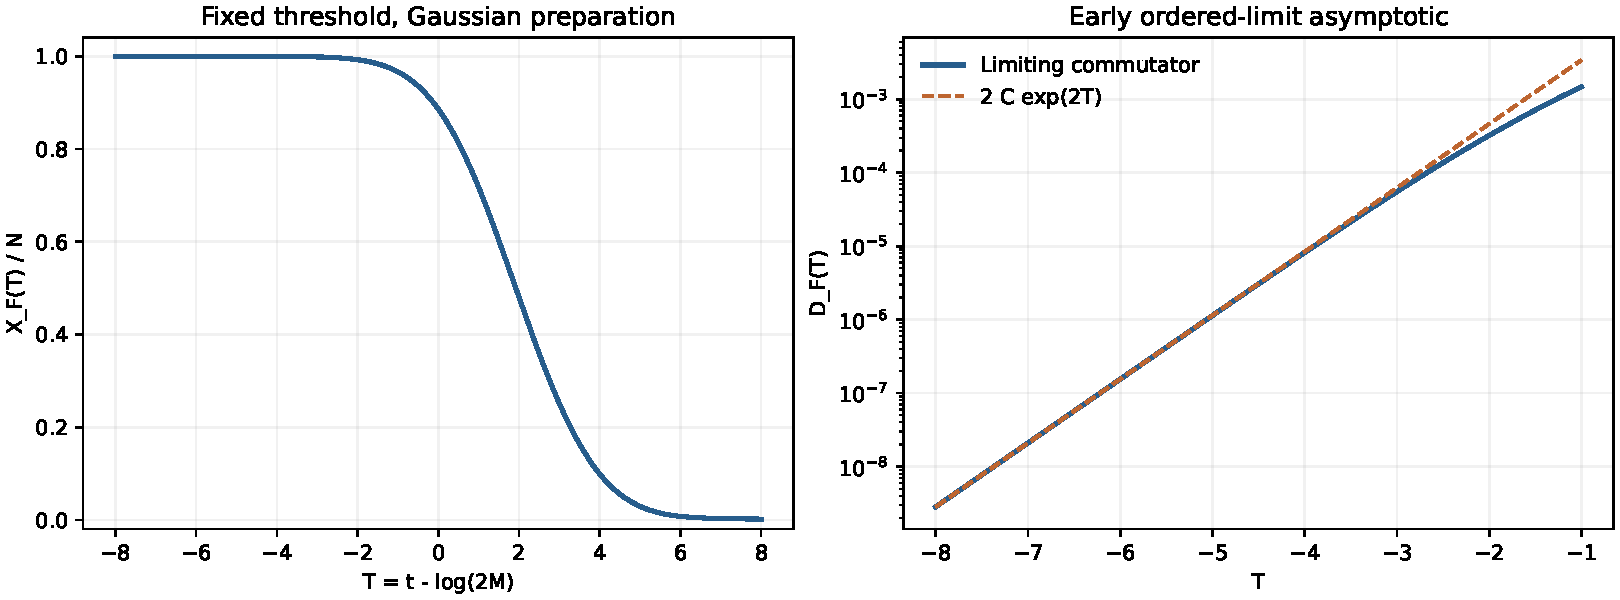
\includegraphics[width=.94\linewidth]{../results/stage3/preparation/fixed-curve.pdf}
 \caption{Fixed-threshold Gaussian limiting curve for $\nu=0.6$,
 $\sigma=1$. The right panel compares the commutator norm with its
 proven ordered-limit early asymptotic. Displayed curves have empirical
 quadrature checks; they are not finite-$M$ data.}
 \label{fig:prep-fixed}
\end{figure}
